\documentclass[runningheads]{llncs}
\usepackage[T1]{fontenc}
\usepackage{amsmath, amssymb, graphics, graphicx}
\usepackage{color}
\usepackage{xcolor}
\usepackage{tikz}
\usetikzlibrary{positioning, calc, shapes, fit}
\usetikzlibrary{positioning, shapes.geometric, shapes, fit, arrows, decorations.markings, arrows.meta}

\begin{document}

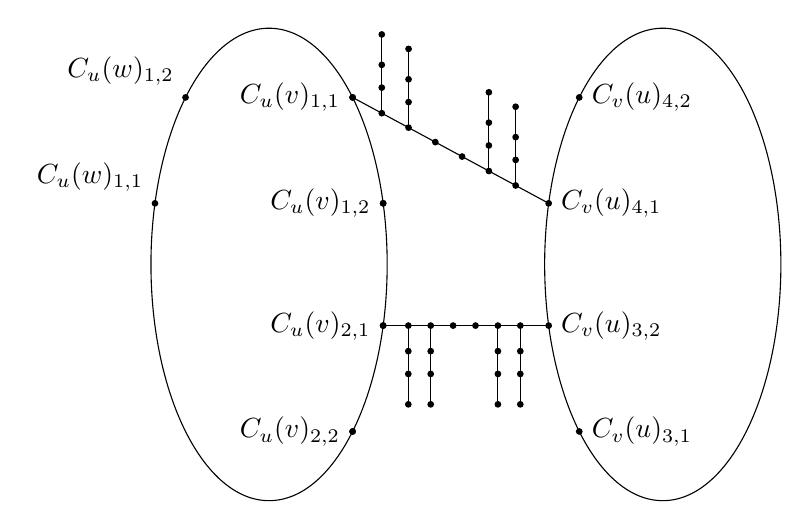
\begin{tikzpicture}
	\tikzset{
		vx/.style={draw, circle, inner sep=0pt, outer sep=0pt, fill, minimum size=2pt}
	}
	\def\u{1}
        \def \a{1.5}
        \def \b{3}
	\draw (0,0) ellipse (1.5 and 3);
	\node[vx] at ($(0,0)+(45:1.5 and 3)$)(a11){};
	\node[vx] at ($(0,0)+(15:1.5 and 3)$)(a12){};
	\node[vx] at ($(0,0)+(-15:1.5 and 3)$)(a21){};
	\node[vx] at ($(0,0)+(-45:1.5 and 3)$)(a22){};
	
	\node[vx, label=left:$C_u(v)_{1,1}$](a11) at ($(0,0)+(45:1.5 and 3)$){};	
	\node[vx, label=left:$C_u(v)_{1,2}$](a12) at ($(0,0)+(15:1.5 and 3)$){};
	\node[vx, label=left:$C_u(v)_{2,1}$](a21) at ($(0,0)+(-15:1.5 and 3)$){};
	\node[vx, label=left:$C_u(v)_{2,2}$](a22) at ($(0,0)+(-45:1.5 and 3)$){};
	\draw (5,0) ellipse (1.5 and 3);
	\node[vx, label=right:$C_v(u)_{4,2}$](b11) at ($(5,0)+(135:1.5 and 3)$){};	
	\node[vx, label=right:$C_v(u)_{4,1}$](b12) at ($(5,0)+(165:1.5 and 3)$){};
	\node[vx, label=right:$C_v(u)_{3,2}$](b21) at ($(5,0)+(195:1.5 and 3)$){};
	\node[vx, label=right:$C_v(u)_{3,1}$](b22) at ($(5,0)+(225:1.5 and 3)$){};

	\draw (a11) edge node foreach \i in {1,...,6}[pos=0.14*\i, vx](c\i){} (b12);
	\draw (a21) edge node foreach \i in {1,...,6}[pos=0.14*\i, vx](d\i){}(b21);
	\foreach \i in {1,2,5,6}
	{
		\draw (c\i)-- ++(0, \u) node foreach \i in {0.3, 0.6, 1}[pos=\i, vx]{};	
		\draw (d\i)-- ++(0, -\u) node foreach \i in {0.3, 0.6, 1}[pos=\i, vx]{};
	}
	\node[vx, label=above left:$C_u(w)_{1,2}$](e11) at ($(0,0)+(135:1.5 and 3)$){};
	\node[vx, label=above left:$C_u(w)_{1,1}$](e12) at ($(0,0)+(165:1.5 and 3)$){};
\end{tikzpicture}

\end{document}